% !TeX encoding = UTF-8
% !TeX program = xelatex
% !TeX spellcheck = en_US

\documentclass[a4paper]{ltxdoc}
\usepackage{amsmath}
\usepackage[UTF8]{ctex}
\usepackage{unicode-math}
\usepackage{caption}
\usepackage{booktabs}
\usepackage{xcolor}
\usepackage{array}
\usepackage{listings}
\usepackage[perpage]{footmisc}
\usepackage{hypdoc}
\usepackage{geometry}
\usepackage{endnotes}
\usepackage{graphicx}
% \usepackage[multiple]{endnotes}
\usepackage{multicol}
\usepackage{blindtext}
\geometry{a4paper, scale=0.85}
\newenvironment{Figure}
{\par\medskip\noindent\minipage{\linewidth}}
{\endminipage\par\medskip}

\title{实验报告\\磁力摆}
\author{少年班学院\\马天开 PB21000030(5号)}
\date{\today}

\begin{document}
\begin{multicols}{2}
    \maketitle
    \section{实验目的}

    理解小磁针在地磁场中运动的特征,掌握测量局部地磁场的方法。设计试验方案测量磁力摆的磁矩和转动惯量,掌握两小磁针耦合运动规律。

    技能方面,掌握基本的电磁学实验技能和电学仪器的使用,锻炼运用刚体力学和电磁学知识,通过变形物理公式,培养数据处理能力。

    \section{实验器材}

    高灵敏度特斯拉计(量程:$0-300mT,\Delta = 0.01mT$)、\textit{Helmholtz}线圈、磁力摆两个、直流电源,质量相同的配重螺母两个、米尺、秒表。

    高灵敏度特斯拉计精度:$0.01mT$,米尺精度:$\Delta = 0.1cm$,秒表精度:$\Delta = 0.01s$

    \section{实验原理}

    \subsection{磁力摆的运动}

    当磁力摆偏离平衡位置角度小于$\theta \leq 5^{\circ}$时,磁力摆的运动方程为:
    \begin{equation}
        \dfrac{d^2\theta}{dt^2} = -\dfrac{mB}{J}\theta
    \end{equation}

    其中,$m$为磁力摆的磁矩,$J$为磁力摆的转动惯量,$B$为所在位置磁感应强度。

    上面的方程是简谐运动方程,一般解的周期计算为:
    \begin{equation}
        T = 2\pi \sqrt{\dfrac{J}{mB}}
        \label{eq:T}
    \end{equation}
    \subsection{\textit{Helmholtz}线圈}
    \textit{Helmholtz}线圈是一对彼此平行且连通的共轴圆形线圈组,每组$N$匝,电流方向一致。
    当线圈之间的距离$a$恰好等于圆形线圈的半径$R$时,两线圈中点附近的磁场近似于均匀磁场,磁感应强度为:

    \begin{equation}
        B_I = (\dfrac{4}{5})^{3/2} \dfrac{\mu_0 I}{R} = kI
    \end{equation}

    \subsection{两小磁针的耦合运动}
    当两个小磁针悬挂在相同高度,同向耦合和反向耦合时,震动周期之间存在如下关系:
    \begin{equation}
        \ln (\dfrac 1 2 \mid \omega^2 + \omega^{*^2} \mid) = -\beta \ln L + \ln (\alpha\cdot m^2)
    \end{equation}

    \section{实验方法}

    \begin{itemize}
        \item \textit{Helmholtz}线圈参数的测量:打开各仪器电源,首先将特斯拉计调零。打开电源,设置输出电压为$U=30V$,逐渐调整电流$I$的大小,($I<1A$),将特斯拉计测量端放置在垂直于磁感线的方向上。记录$I-B$值的大小。(共8组)
        \item 测量局部地磁场水平分量的大小:首先确定通入电流后线圈产生的磁场方向和地磁场方向平行,方法如下:在未通电的情况下,悬挂一小磁针。此时小磁针所指方向为地磁场的水平分量方向。以此方向平行放置\textit{Helmholtz}线圈,此时调整线圈中通入电流大小,若随着电流增大,摆动周期逐渐减小,说明线圈摆放方向与地磁场方向相同。相反的表现是:随着电流增大,摆动周期先增大后减小(反映叠加磁场从变弱到变强)。控制电流大小$I<0.1A$,随着电流变化,记录磁针摆动周期的变化(100次)。
        \item 测量转动惯量及磁矩:调整电流大小$I=0.02A$,测量磁针摆动周期(100次),并测量螺帽到悬线长度。
        \item 地磁场中耦合现象的观察:将两个小磁针同高度悬挂,分别令他们同向耦合、反向耦合,记录他们的摆动周期($\omega$和$\omega^{*}$)。同时和小磁针单独运动的周期对比,比较三者关系。
        \item 地磁场中耦合磁针运动的测量:将两个小磁针同高度悬挂,分别测量同相位周期$\omega$和反相位周期$\omega^{*}$,记录两者随着磁针间水平距离$L$之间的变化。
    \end{itemize}

    \section{实验数据}
    \subsection{线圈参数的测量\\($U=30V$)}

    \begin{tabular}{|c|c|c|c|c|c|}
        \hline
        I/A  & 0.1  & 0.2  & 0.3  & 0.4  & 0.5  \\\hline
        B/mT & 0.47 & 0.91 & 1.37 & 1.83 & 2.29 \\\hline
        I/A  & 0.6  & 0.7  & 0.8  & 0.9  & 1.0  \\\hline
        B/mT & 2.76 & 3.23 & 3.71 & 4.17 & 4.64 \\\hline
    \end{tabular}

    \subsection{测量局部地磁场水平分量的大小\\($U=30V$)}

    \begin{tabular}{|c|c|c|c|}
        \hline
        I/A   & $100T_1/s$ & $100T_2/s$ & $100T_3/s$ \\\hline
        0.01  & 67.13      & 67.14      & 67.32      \\\hline
        0.015 & 60.32      & 59.44      & 58.82      \\\hline
        0.02  & 54.07      & 53.35      & 55.77      \\\hline
        0.025 & 49.40      & 48.75      & 48.54      \\\hline
        0.03  & 46.76      & 45.29      & 45.17      \\\hline
        0.035 & 43.90      & 42.79      & 42.46      \\\hline
        0.04  & 40.60      & 40.10      & 40.56      \\\hline
        0.045 & 38.19      & 38.29      & 37.68      \\\hline
    \end{tabular}

    \subsection{测量转动惯量及磁矩\\($U=30V, I = 0.02A$)}

    \begin{tabular}{|c|c|c|c|}
        \hline
        100T/s & 74.00 & 73.54 & 73.42 \\\hline
        d/cm   & 5.60  & 5.61  & 5.60  \\\hline
    \end{tabular}

    \subsection{地磁场中耦合现象的观察}

    \begin{tabular}{|c|c|c|c|}
        \hline
        $100\omega_0/s$   & 107.28 & 107.03 & 107.23 \\\hline
        $100\omega/s$     & 65.88  & 65.57  & 65.63  \\\hline
        $100\omega^{*}/s$ & 102.48 & 104.75 & 103.46 \\\hline
    \end{tabular}

    \subsection{地磁场中耦合磁针运动的测量}

    \begin{tabular}{|c|c|c|}
        \hline
        L/cm & $100\omega/s$ & $100\omega^{*}/s$ \\\hline
        23.5 & 80.19         & 92.46             \\\hline
        25.0 & 83.70         & 97.34             \\\hline
        26.5 & 84.03         & 98.39             \\\hline
        28.0 & 91.93         & 102.60            \\\hline
        29.5 & 93.23         & 103.46            \\\hline
        31.0 & 94.00         & 105.27            \\\hline
    \end{tabular}

    \section{数据处理}

    \subsection{线圈参数的测量}

    对$I-B$进行线性拟合,得到:
    \begin{Figure}
        \centering
        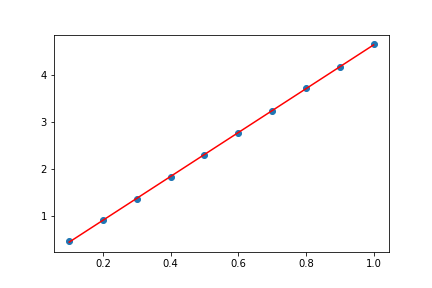
\includegraphics[scale=0.5]{img/data_1.png}
    \end{Figure}
    \begin{equation}
        \left\{
        \begin{aligned}
            B        & = 4.65\cdot I - 0.02                                                         \\
            S_\kappa & = \kappa\cdot \sqrt{\dfrac{\dfrac {1} {R^2} -1}{n-2}} = 1.471 \times 10^{-2} \\
        \end{aligned}
        \right.
    \end{equation}

    \begin{equation}
        \left\{
        \begin{aligned}
            u_{A\kappa}       & = S_\kappa \times t_p = 0.15 mT/A \\
            \therefore \kappa & = 4.65 \pm 0.15 mT/A              \\
        \end{aligned}
        \right.
    \end{equation}

    \subsection{测量局部地磁场水平分量的大小}

    利用公式~\ref{eq:T}~,并计算到地磁场,得到:
    \begin{equation}
        I = \dfrac {1} {\kappa} (\dfrac{2\pi J}{m} \cdot \dfrac {1}{T^2} - B_0)
    \end{equation}

    对$\dfrac{1}{T^2} - I$进行线性拟合,得到:

    \begin{Figure}
        \centering
        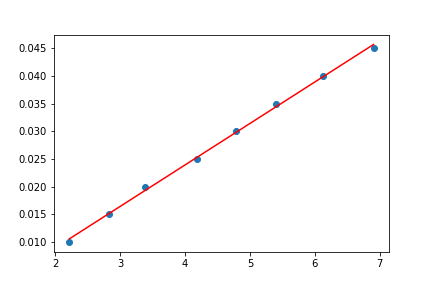
\includegraphics[scale=0.5]{img/data_2.png}
    \end{Figure}

    \begin{equation}
        \left\{
        \begin{aligned}
            B_0           & = \kappa \cdot b = 27.98 mT                            \\
            U_{B_0} / B_0 & = \sqrt{(U_\kappa / \kappa)^2 + (U_b / b)^2} = 0.23 mT \\
        \end{aligned}
        \right.
    \end{equation}

    \begin{equation}
        \therefore B_0 = 27.98 \pm 0.23 mT
    \end{equation}

    \subsection{测量转动惯量及磁矩}

    对公式~\ref{eq:T}~,考虑到转动惯量的变化,符合以下两个公式:
    \begin{equation}
        \left\{
        \begin{aligned}
            J_0                     & = (\dfrac{T_0}{2\pi})^2 \cdot mB \\
            J_0 + \frac 1 2 m_0 d^2 & = (\dfrac{T}{2\pi})^2 \cdot mB   \\
        \end{aligned}
        \right.
    \end{equation}

    因此有,

    \begin{equation}
        m = \dfrac{2\pi^2m_0d^2}{(T^2 - T_0^2)\cdot B}
    \end{equation}

    同时,计算不确定度为:

    \begin{equation}
        \begin{aligned}
            (U_m / m)^2 = (U_{m_0}/m_0)^2 + (U_d/d)^2 + 2(U_T/T)^2 \\
            + 2(U_{T_0}/{T_0})^2 + (U_B/B)^2
        \end{aligned}
    \end{equation}

    计算得到:
    \begin{equation}
        \begin{aligned}
            m   & = 1.75 \pm 0.14 A\cdot m^2  \\
            J_0 & = 1.19 \pm 0.05 kg\cdot m^2 \\
        \end{aligned}
    \end{equation}
    \subsection{地磁场中耦合现象的观察}

    根据测量结果:
    \begin{equation}
        \omega < \omega^{*} < \omega_0
    \end{equation}

    \subsection{地磁场中耦合磁针运动的测量}

    对$\ln L - \ln (\dfrac 1 2 \mid \omega^2 + \omega^{*^{2}} \mid)$进行线性拟合,得到:

    \begin{Figure}
        \centering
        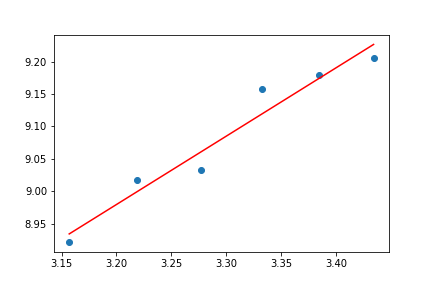
\includegraphics[scale=0.5]{img/data_3.png}
    \end{Figure}

    因此计算出$\beta = -1.057, \alpha = 88.037$

    \section{实验结论}
    \subsection{结果}
    见数据处理部分。
    \subsection{思考题}
    \begin{itemize}
        \item 如何利用作图法或最小二乘法求得局部地磁场的水平分量?\\附加磁场的强度,随电流增强成线性变化,因此测算周期零点的周期,便可得到地磁场的水平分量
        \item 如何说明两小磁针耦合运动“拍频”与那些物理量有关?\\与外加磁场、距离、小磁针的磁矩相关。
    \end{itemize}
\end{multicols}
\end{document}